\documentclass[11pt,a4paper]{article}

\usepackage[utf8]{inputenc}
\usepackage[T1]{fontenc}
\usepackage[a4paper,margin=2.5cm]{geometry}
\usepackage[table]{xcolor}
\usepackage{titlesec}
\usepackage{fancyhdr}
\usepackage{enumitem}
\usepackage{tabularx}
\usepackage{longtable}
\usepackage{booktabs}
\usepackage{listings}
\usepackage[most]{tcolorbox}
\usepackage{hyperref}
\usepackage{parskip}
\usepackage{helvet}
\usepackage{amsmath}
\usepackage{amssymb}
\usepackage{lastpage}
\usepackage{tikz}
\usetikzlibrary{shapes.geometric, arrows.meta, positioning, fit, backgrounds, calc}
\renewcommand{\familydefault}{\sfdefault}

\definecolor{accent}{HTML}{1F4E78}
\definecolor{accentlight}{HTML}{DDEBF7}
\definecolor{codebg}{HTML}{F2F2F2}
\definecolor{codeframe}{HTML}{CCCCCC}
\definecolor{tablehead}{HTML}{1F4E78}
\definecolor{warnbg}{HTML}{FBEAEA}
\definecolor{warnframe}{HTML}{B33A3A}

\titleformat{\section}{\color{accent}\Large\bfseries}{\thesection.}{0.5em}{}
\titleformat{\subsection}{\color{accent}\large\bfseries}{\thesubsection}{0.5em}{}
\titleformat{\subsubsection}{\color{accent}\normalsize\bfseries}{\thesubsubsection}{0.5em}{}
\titlespacing*{\section}{0pt}{18pt}{8pt}
\titlespacing*{\subsection}{0pt}{14pt}{6pt}

\pagestyle{fancy}
\fancyhf{}
\renewcommand{\headrulewidth}{0.4pt}
\fancyhead[R]{\small\color{gray}polyN\_pipeline --- User \& Methodology Manual}
\fancyfoot[C]{\small\color{gray}Page \thepage\ / \pageref{LastPage}}

\lstdefinestyle{shell}{
  backgroundcolor=\color{codebg}, basicstyle=\ttfamily\small, breaklines=true,
  frame=single, rulecolor=\color{codeframe}, framesep=6pt,
  xleftmargin=6pt, xrightmargin=6pt, aboveskip=8pt, belowskip=10pt,
}
\lstset{style=shell}

\newtcolorbox{remark}[1][Remark]{
  colback=accentlight, colframe=accent, boxrule=0pt, leftrule=3pt,
  arc=0pt, outer arc=0pt, left=8pt, right=8pt, top=5pt, bottom=5pt,
  fonttitle=\bfseries, coltitle=white, colbacktitle=accent, title={#1}}

\newtcolorbox{finding}[1][Empirical finding]{
  colback=warnbg, colframe=warnframe, boxrule=0pt, leftrule=3pt,
  arc=0pt, outer arc=0pt, left=8pt, right=8pt, top=5pt, bottom=5pt,
  fonttitle=\bfseries, coltitle=white, colbacktitle=warnframe, title={#1}}

\newcolumntype{K}{>{\ttfamily\small}p{3.6cm}}
\newcolumntype{D}{>{\ttfamily\small}p{2.6cm}}
\newcolumntype{T}{p{7.2cm}}

\hypersetup{colorlinks=true, linkcolor=accent, urlcolor=accent, citecolor=accent,
  pdftitle={polyN pipeline Manual}, pdfauthor={Gilles Frapper}}

\begin{document}

\begin{titlepage}
\centering
\vspace*{2.5cm}
{\Huge\bfseries\color{accent}polyN\_pipeline\par}
\vspace{0.5em}
{\Large User \& Methodology Manual\par}
\vspace{2em}
{\itshape\large Topology generation (isolobal / random / MAYGEN / geng) $\rightarrow$
GFN2-xTB optimization $\rightarrow$ frequency verification\par}
{\itshape\large $\rightarrow$ per-charge-family convex hulls\par}
\vspace{3em}
{\large Application: screening of neutral, cationic, and anionic
polynitrogen allotropes (N$_2$--N$_{16}$)\par}
\vspace{3em}
{\bfseries Gilles Frapper\par}
{\small IC2MP (UMR 7285 CNRS), University of Poitiers\par}
\vfill
{\small\color{gray}Version 3.0 --- July 2026\par}
\end{titlepage}

\tableofcontents
\newpage

% =============================================================================
\section{Introduction}
% =============================================================================

\texttt{polyN\_pipeline} builds an energetic stability map for a set of
polynitrogen allotrope stoichiometries, studied separately by charge state
(neutral, cation, anion). The complete workflow chains together:

\begin{enumerate}[itemsep=2pt]
  \item generation of candidate molecular topologies, from one or several
    interchangeable sources (\S\ref{sec:generators})---isolobal
    substitution (default), random graph sampling, MAYGEN enumeration, or exhaustive geng (nauty) enumeration;
  \item an initial 3D geometry for each topology (RDKit ETKDGv3);
  \item GFN2-xTB geometry optimization in two stages: a cheap
    \emph{checkpoint} to rank candidates, then precise refinement of the
    best ones only (\S\ref{sec:checkpoint});
  \item selection of the lowest-energy structures per stoichiometry;
  \item \textbf{frequency verification}: confirmation that each retained
    structure is a genuine local minimum (all real frequencies), with
    automatic relaxation of any saddle point toward the true nearby minimum
    (\S\ref{sec:frequency});
  \item formation energies and \textbf{a separate convex hull per charge
    family}, each with its own energy reference (\S\ref{sec:references}).
\end{enumerate}

All structures are treated as isolated (non-periodic) molecules. Geometry
optimization is performed entirely at the GFN2-xTB level through the
\texttt{tblite} Python/ASE interface; there is no external tight-binding or
DFT re-optimization step in this version.

\begin{remark}
This version is intended not only to find the most stable species, but also
to assemble a clean, minimum-verified dataset of polynitrogen structures
(neutral, cationic, anionic) suitable for training a generative model. The
selection settings can therefore be widened (large \texttt{top\_n}) to keep
many structures per stoichiometry rather than only the single best.
\end{remark}

% =============================================================================
\section{Workflow overview}
% =============================================================================

The pipeline runs five stages, from topology generation (one or more of the
three interchangeable sources) to a separate convex hull per charge family.

\begin{center}
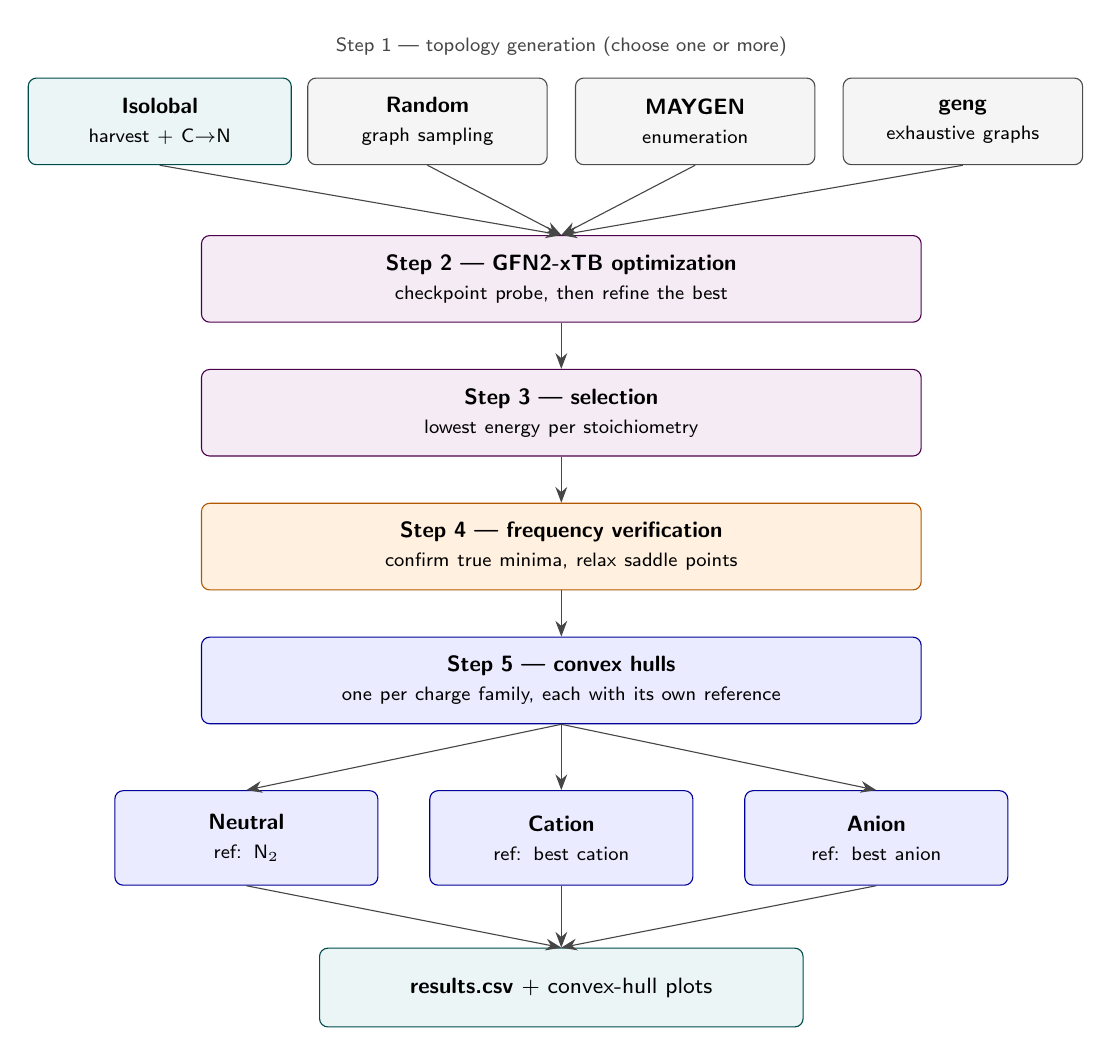
\begin{tikzpicture}[
  font=\footnotesize,
  gen/.style   ={rectangle, rounded corners=3pt, draw=teal!60!black, fill=teal!8,
                 text width=3.2cm, align=center, minimum height=11mm, inner sep=2pt},
  genb/.style  ={rectangle, rounded corners=3pt, draw=gray!60!black, fill=gray!8,
                 text width=2.9cm, align=center, minimum height=11mm, inner sep=2pt},
  core/.style  ={rectangle, rounded corners=3pt, draw=violet!60!black, fill=violet!8,
                 text width=9cm, align=center, minimum height=11mm, inner sep=2pt},
  freq/.style  ={rectangle, rounded corners=3pt, draw=orange!70!black, fill=orange!12,
                 text width=9cm, align=center, minimum height=11mm, inner sep=2pt},
  hull/.style  ={rectangle, rounded corners=3pt, draw=blue!60!black, fill=blue!8,
                 text width=9cm, align=center, minimum height=11mm, inner sep=2pt},
  fam/.style   ={rectangle, rounded corners=3pt, draw=blue!60!black, fill=blue!8,
                 text width=3.2cm, align=center, minimum height=12mm, inner sep=2pt},
  pout/.style  ={rectangle, rounded corners=3pt, draw=teal!60!black, fill=teal!8,
                 text width=6cm, align=center, minimum height=10mm, inner sep=2pt},
  arr/.style   ={-{Stealth[length=2mm]}, draw=gray!55!black, thin},
]

% --- Row 1: four generators (y = 0) ---
\node[gen]  (iso) at (-5.1, 0)   {\textbf{Isolobal}\\[1pt]{\scriptsize harvest + C$\to$N}};
\node[genb] (rnd) at (-1.7, 0)   {\textbf{Random}\\[1pt]{\scriptsize graph sampling}};
\node[genb] (may) at ( 1.7, 0)   {\textbf{MAYGEN}\\[1pt]{\scriptsize enumeration}};
\node[genb] (gen) at ( 5.1, 0)   {\textbf{geng}\\[1pt]{\scriptsize exhaustive graphs}};

% --- Core column (centered x = 0) ---
\node[core] (opt) at (0, -2.0)   {\textbf{Step 2 --- GFN2-xTB optimization}\\[1pt]{\scriptsize checkpoint probe, then refine the best}};
\node[core] (sel) at (0, -3.7)   {\textbf{Step 3 --- selection}\\[1pt]{\scriptsize lowest energy per stoichiometry}};
\node[freq] (frq) at (0, -5.4)   {\textbf{Step 4 --- frequency verification}\\[1pt]{\scriptsize confirm true minima, relax saddle points}};
\node[hull] (hul) at (0, -7.1)   {\textbf{Step 5 --- convex hulls}\\[1pt]{\scriptsize one per charge family, each with its own reference}};

% --- Row: three families (y = -9.1) ---
\node[fam] (neu) at (-4.0, -9.1) {\textbf{Neutral}\\[1pt]{\scriptsize ref: N$_2$}};
\node[fam] (cat) at ( 0.0, -9.1) {\textbf{Cation}\\[1pt]{\scriptsize ref: best cation}};
\node[fam] (ani) at ( 4.0, -9.1) {\textbf{Anion}\\[1pt]{\scriptsize ref: best anion}};

% --- Output ---
\node[pout] (res) at (0, -11.0)  {\textbf{results.csv} + convex-hull plots};

% --- Arrows ---
\draw[arr] (iso.south) -- (opt.north);
\draw[arr] (rnd.south) -- (opt.north);
\draw[arr] (may.south) -- (opt.north);
\draw[arr] (gen.south) -- (opt.north);
\draw[arr] (opt) -- (sel);
\draw[arr] (sel) -- (frq);
\draw[arr] (frq) -- (hul);
\draw[arr] (hul.south) -- (neu.north);
\draw[arr] (hul.south) -- (cat.north);
\draw[arr] (hul.south) -- (ani.north);
\draw[arr] (neu.south) -- (res.north);
\draw[arr] (cat.south) -- (res.north);
\draw[arr] (ani.south) -- (res.north);

\node[text=gray!55!black] at (0, 0.95) {\scriptsize Step 1 --- topology generation (choose one or more)};
\end{tikzpicture}
\end{center}

All optimization is performed at the GFN2-xTB level (\texttt{tblite}); there
is no DFT or DFTB re-optimization step. Each stage is detailed in the
sections that follow.



\begin{lstlisting}
conda create -n polyN python=3.11 -y
conda activate polyN
conda install -c conda-forge tblite-python rdkit ase pyyaml pandas scipy matplotlib -y
pip install pubchempy    # only for the isolobal harvest generator
# only for the geng generator: nauty's geng executable
#   macOS:  brew install nauty
#   Debian: sudo apt install nauty
\end{lstlisting}

Verify:
\begin{lstlisting}
python3 -c "from tblite.ase import TBLite; from rdkit import Chem; import ase, yaml, pandas; print('OK')"
\end{lstlisting}

\begin{remark}[macOS PATH note]
If \texttt{which python3} points to a Homebrew interpreter instead of your
conda environment, prefix commands with \texttt{\textasciitilde/miniconda3/bin/python3},
or place a \texttt{miniconda3/bin} PATH export at the very end of
\texttt{\textasciitilde/.zshrc}. A stale shell hash table can also mask a
corrected PATH---open a fresh terminal or run \texttt{hash -r}.
\end{remark}

% =============================================================================
\section{Topology generators}
\label{sec:generators}
% =============================================================================

Three complementary topology sources are available, selected with the
\texttt{--generators} option (one or more; combining them yields a richer,
deduplicated candidate pool). The default is \texttt{isolobal}.

\begin{lstlisting}
python3 polyN_pipeline.py --config config.yaml                       # isolobal (default)
python3 polyN_pipeline.py --config config.yaml --generators isolobal random
python3 polyN_pipeline.py --config config.yaml --generators none     # pre-existing inputs
\end{lstlisting}

\subsection{Isolobal substitution (default) --- \texttt{cxhx\_to\_nx.py}}
\label{sec:isolobal}

\subsubsection{The electron-accounting argument}

The substitution rests on a precise isolobal relationship, not a loose shape
analogy. Consider a C--H unit inside a hydrocarbon framework. Formally split
the C--H bond heterolytically: the bonding pair stays on carbon, giving
C$^{-}$ + H$^{+}$. A carbanion C$^{-}$ has 5 valence electrons arranged as
three framework bonds plus one lone pair --- which is \emph{exactly} the
valence configuration of a neutral nitrogen atom. In short:
\[
  \mathrm{C\!-\!H} \;\equiv\; \mathrm{C}^{-} + \mathrm{H}^{+},
  \qquad \mathrm{C}^{-} \;\cong\; \mathrm{N}.
\]
So replacing each C--H by N and removing the hydrogen conserves the $\sigma$
framework and turns the former C--H bonding pair into a nitrogen lone pair.
The mapping generalizes to carbons in any bonding environment. Counting only
bonds to non-hydrogen (framework) neighbors, the formal charge that the new
nitrogen must carry is
\[
  q(\mathrm{C}\rightarrow\mathrm{N})
    = (\text{framework bond order}) - 3.
\]

\begin{itemize}[itemsep=2pt]
  \item A \emph{three-coordinate} CH (framework order 3, e.g.\ a cage or
    aromatic vertex) $\rightarrow$ neutral N. \emph{Example}: tetrahedrane
    C$_4$H$_4$ $\rightarrow$ tetrahedral N$_4$; benzene $\rightarrow$
    hexazine.
  \item A \emph{two-coordinate} $>$CH$_2$ or $=$CH$-$ (framework order 2)
    $\rightarrow$ a bent, two-coordinate N$^{-}$ center --- isolobal with the
    bent nitrogen of azide N$_3^{-}$ or of the pentazolate ring.
    \emph{Example}: cyclopentadiene, whose sp$^3$ CH$_2$ bridges the diene,
    maps cleanly onto the pentazolate anion N$_5^{-}$ --- the CH$_2$ becomes
    the formally negative, two-coordinate ring nitrogen.
  \item A \emph{four-coordinate} carbon (framework order 4) $\rightarrow$ an
    ammonium-like N$^{+}$ center.
\end{itemize}

Because the charge \emph{emerges} from each precursor's bonding pattern
rather than being imposed, scanning a hydrocarbon database populates the
neutral, cation, and anion families simultaneously in a single pass.

\subsubsection{Rejection filters for over-charged species}

A precursor rich in terminal CH$_3$ / CH$_2$ groups maps to a nitrogen
species carrying a large concentrated formal charge (e.g.\ a lone CH$_3$
becomes an N$^{2-}$ center). Such highly charged species are chemically
implausible and are removed by two filters:
\begin{itemize}[itemsep=2pt]
  \item \texttt{--max-abs-charge M}: discards any converted structure whose
    \emph{net} charge exceeds $\pm M$ (default $M=1$, i.e.\ keep only
    neutral, $+1$, $-1$).
  \item A final \textbf{purity gate}: after substitution and hydrogen
    removal, any structure that still contains a hydrogen atom is rejected
    outright. This is the minimal, infallible criterion --- it silently
    discards precursors whose mapping would leave orphaned hydrogens, while
    keeping every genuinely clean conversion (pentazolate included).
\end{itemize}

\subsubsection{Which database, and what kind of structures}

The harvester \texttt{harvest\_hydrocarbons.py} queries \textbf{PubChem} (via
\texttt{pubchempy}) for hydrocarbons of exact formula C$_x$H$_y$ across a
range of carbon counts. PubChem is a repository of \textbf{real,
experimentally-reported compounds}, so the resulting nitrogen topologies
descend from hydrocarbon scaffolds that actually exist in the chemical
literature --- as opposed to purely theoretical enumeration. This is the
method's strength (chemically-motivated seeds) and its limitation (it only
covers catalogued scaffolds, a smaller, non-exhaustive set).

\begin{lstlisting}
python3 harvest_hydrocarbons.py --min-c 4 --max-c 16 -o hydrocarbons.smi
python3 cxhx_to_nx.py --smiles-file hydrocarbons.smi --max-abs-charge 1 -o seeds/
\end{lstlisting}

Harvester options (\texttt{-h}): \texttt{--min-c}/\texttt{--max-c} (carbon
range), \texttt{--max-per-formula} (cap per exact formula, to bound run
time), and \texttt{--resume} (continue from a checkpoint after an
interruption --- the harvest records each completed formula, and a hard
network timeout prevents the indefinite hangs that a raw PubChem request can
otherwise cause). Other public sources of \emph{experimental} hydrocarbon
structures (ChEMBL, the crystallographic databases) or of \emph{theoretical}
ones (GDB, QM9) could be substituted by feeding their SMILES to
\texttt{cxhx\_to\_nx.py --smiles-file}; only the PubChem harvester is
provided out of the box.

\begin{finding}[Validation]
The substitution reproduces known results exactly: tetrahedrane and
cyclobutadiene give precisely the two N$_4$ isomers found independently by
MAYGEN; cyclopentadiene gives the pentazolate anion N$_5^{-}$; benzene gives
hexazine; norbornadiene (C$_7$H$_8$) gives an N$_7^{-}$ anion --- a candidate
discovered without ever targeting it.
\end{finding}

\subsection{Random graph sampling --- \texttt{random\_structure\_generator.py}}
\label{sec:random}

\subsubsection{A molecule as a graph}

In graph terms a polynitrogen molecule is a graph whose \textbf{vertices} are
nitrogen atoms and whose \textbf{edges} are N--N bonds; a double or triple
bond is a multi-edge (two or three parallel edges between the same pair of
vertices). The valence of an atom is its vertex degree counted with edge
multiplicity. A valid neutral topology is then a connected graph in which
every vertex has total degree 3.

\begin{center}
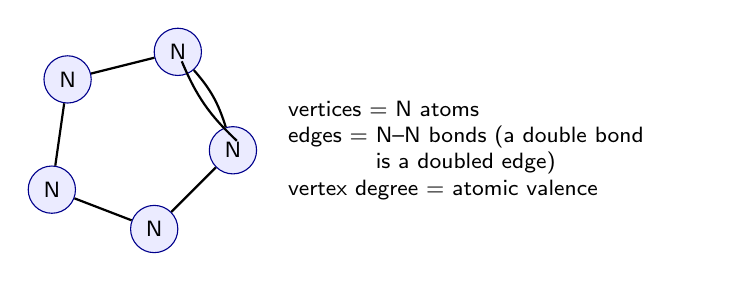
\begin{tikzpicture}[font=\footnotesize,
  N/.style={circle, draw=blue!55!black, fill=blue!8, minimum size=6mm, inner sep=0pt}]
% a small illustrative N5-like graph: ring with one double bond
\node[N] (a) at (0,0)   {N};
\node[N] (b) at (1.4,0.35) {N};
\node[N] (c) at (2.1,-0.9) {N};
\node[N] (d) at (1.1,-1.9) {N};
\node[N] (e) at (-0.2,-1.4) {N};
\draw[thick] (a)--(b);
\draw[thick] (b) to[bend left=12] (c);
\draw[thick] ($(b)+(0.05,-0.12)$) to[bend right=12] ($(c)+(0.05,0.12)$); % 2nd edge = double bond
\draw[thick] (c)--(d);
\draw[thick] (d)--(e);
\draw[thick] (e)--(a);
\node[align=left, text width=5.2cm] at (5.4,-0.9)
  {\footnotesize vertices = N atoms\\
   edges = N--N bonds (a double bond\\ \hphantom{edges = }is a doubled edge)\\
   vertex degree = atomic valence};
\end{tikzpicture}
\end{center}

The generator draws such graphs at random using the \textbf{configuration
model} (``stub matching''): each atom is given a number of half-edges
(stubs) equal to its target valence, the stubs are paired at random, and a
short repair step restores connectivity if needed. A per-atom valence
sequence, or a target net charge with randomly placed low-valence (terminal,
$-1$) and high-valence (hub, $+1$) defect centers, lets the charged families
be sampled directly.

\begin{lstlisting}
python3 random_structure_generator.py -n 16 -k 2000 --valence 3 -o N16.smi
python3 random_structure_generator.py -n 9 -k 100 --target-charge -1 -o N9_anion.smi
\end{lstlisting}

\subsubsection{Approximate size of the space}

The number of distinct neutral valence-3 topologies grows steeply with $N$
(2, 6, 20, 91, 509, 3608 for N$_4$ through N$_{14}$). Random sampling
sidesteps having to enumerate them all: it draws a fixed number $k$ of
distinct graphs regardless of how large the underlying space is.

\begin{finding}[A hard topological constraint]
For a connected graph in which every atom has exactly 3 bonds, the number of
independent rings (the cyclomatic number) is fixed by Euler's formula:
\[
  \text{rings} = \text{edges} - \text{vertices} + 1 = \frac{3N}{2} - N + 1
    = \frac{N}{2} + 1.
\]
This is independent of the construction method. At $N=16$, nine independent
rings are mandatory in any neutral valence-3 molecule --- large discrete
polynitrogen molecules are therefore necessarily caged/fused, consistent with
the extended covalent networks of high-pressure polymeric nitrogen. The high
3D-embedding failure rate at large $N$ reflects this genuine structural
difficulty, not a numerical artifact; the pragmatic response is to
over-generate (near-zero cost) to compensate.
\end{finding}

\subsubsection{The RDKit hydrogen-saturation problem}

The generator builds each graph in RDKit. RDKit's default valence model
assumes an organic context and will \textbf{silently add an implicit hydrogen}
to any nitrogen left below valence 3 --- precisely the automatic saturation
we do \emph{not} want, since it would turn a bare N$_x$ topology into a
contaminated N$_x$H$_y$ species. This was the source of a real contamination
bug (hydrogens appearing in supposedly pure anion structures). The fix, applied
throughout, is twofold:
\begin{itemize}[itemsep=2pt]
  \item set \texttt{SetNoImplicit(True)} on every generated atom, so RDKit
    never completes a valence with a phantom hydrogen, whether or not a formal
    charge is also assigned;
  \item run the same purity gate as the isolobal generator --- reject any
    structure that still contains a hydrogen after construction.
\end{itemize}
The companion tool \texttt{check\_xyz\_purity.py} scans any set of
\texttt{.xyz} files and flags those containing an element other than the
expected one, as a standing guard against this class of error.

\subsection{MAYGEN enumeration --- external jar}
\label{sec:maygen}

MAYGEN (Yirik, Sorokina, Steinbeck, \emph{J.\ Cheminform.} 2021) is an
open-source, pure-Java constitutional-isomer generator built on the CDK. The
following summarizes its documented methodology:
\begin{itemize}[itemsep=2pt]
  \item It takes a molecular formula as input and generates \emph{all}
    non-isomorphic constitutional isomers of that formula.
  \item It uses the \textbf{orderly generation} principle from algorithmic
    group theory: canonical graphs are constructed \emph{during} generation,
    so the enumeration is exhaustive and isomorphism-free without any
    subsequent deduplication filtering step.
  \item It makes \textbf{no assumptions about chemical stability} --- for
    small ring systems this can yield strained or unusual structures.
  \item Performance (per the paper's benchmarks): roughly 47$\times$ faster
    than the open-source PMG generator, and about 3$\times$ slower than the
    closed-source MOLGEN.
\end{itemize}
In this pipeline MAYGEN is used for the neutral families only. Set
\texttt{generators.maygen.jar} to the MAYGEN \texttt{.jar} path. Note the
combinatorial wall: enumeration becomes intractable by N$_{16}$ (over 10
hours without completing), which is exactly why the random generator
(\S\ref{sec:random}) exists as an alternative at large sizes.

\subsection{Exhaustive enumeration via geng (nauty) --- \texttt{geng\_enumerate.py}}
\label{sec:geng}

The fourth generator enumerates topologies \emph{exhaustively} rather than by
sampling or by substituting an existing scaffold. It builds on
\texttt{geng} from the nauty package (McKay \& Piperno), which produces every
connected, non-isomorphic simple graph on $N$ vertices. For each such graph
the generator then explores bond-order assignments (single / double / triple)
on the edges, and derives each nitrogen's formal charge from its bonding
pattern.

\subsubsection{Why this complements the other three}

\begin{itemize}[itemsep=2pt]
  \item Unlike the \emph{random} generator, it is \textbf{exhaustive} over
    graph topologies (up to an optional sampling cap): for a given $N$ no
    connected topology is missed.
  \item Unlike \emph{MAYGEN}, which enumerates constitutional isomers of a
    fixed formula and does not vary bond order to produce charges, geng gives
    the bare connected graphs and \emph{we} distribute the bond orders --- so
    the neutral, cation, and anion families all emerge from the \textbf{same
    graph set} in one pass.
\end{itemize}

\subsubsection{Formal charges assigned at the graph stage}

This is the methodological crux, and the reason a naive version of this idea
fails. A nitrogen atom has 5 valence electrons and, with one lone pair by
default, a neutral valence of 3. With total incident bond order $b$ at an
atom, the formal charge is
\[
  q = b - 3
  \qquad (b=2 \to -1 \text{ bent N};\; b=3 \to 0;\; b=4 \to +1).
\]
This is the \emph{same} accounting the isolobal generator uses, so the two
sources are chemically consistent and deduplicate cleanly. Crucially, the
charge is written onto the RDKit atom (\texttt{SetFormalCharge}) together with
\texttt{SetNoImplicit(True)} \textbf{before the molecule is sanitized}. If the
charge were left off, RDKit would see, say, a four-bonded neutral nitrogen ---
an illegal valence --- and either reject the structure outright or (for an
under-valent nitrogen) silently complete it with a phantom hydrogen, turning a
pure N$_x$ cluster into a contaminated N$_x$H$_y$ species. Assigning the charge
at the graph stage is what makes the enumeration produce clean cations and
anions at all. A final purity gate rejects any structure that is not pure
nitrogen, as a defensive backstop.

\begin{lstlisting}
python3 geng_enumerate.py -n 10 --max-abs-charge 1 -o seeds/
python3 geng_enumerate.py -n 6 --max-graphs 500 --max-abs-charge 1 -o seeds/
\end{lstlisting}

\begin{finding}[Combinatorial cost]
Two factors compound: the number of connected graphs on $N$ vertices (already
$1.17\times10^{7}$ at $N=10$) and, for each graph with $m$ edges, the
$3^{m}$ bond-order assignments. Early per-vertex pruning on the
bond-order-sum ceiling ($\le 4$) removes most branches, but for $N \gtrsim 9$
a \texttt{--max-graphs} cap is recommended. Validation reproduces the
textbook ions directly: the azide anion appears as
\texttt{[N-]=[N+]=[N-]}, and enumerating the five-membered ring yields the
pentazolate \texttt{n1nn[n-]n1} --- both with zero hydrogens.
\end{finding}

\subsection{Combining generators and removing duplicates}
\label{sec:dedup}

The four sources overlap --- the same topology can be produced by more than
one. When \texttt{--generators} lists several sources (or a single source
with several conformers per isomer), duplicates are removed automatically:
two candidates with the same formula and charge whose optimized energies
agree within \texttt{dedup\_tol\_kcalmol} (default 0.5) are treated as the
same structure, and the lowest-energy representative is kept. Deduplication
runs \textbf{after optimization} (energies exist) and \textbf{again after
frequency verification}, because following imaginary modes can collapse two
initially-distinct structures onto the same minimum.



% =============================================================================
\section{The two-stage optimization strategy}
\label{sec:checkpoint}
% =============================================================================

With thousands of candidates per stoichiometry at large $N$, optimizing all
of them at the precise (\texttt{tight}) GFN2-xTB level is expensive. The
pipeline uses the \textbf{same GFN2-xTB Hamiltonian} at both stages; the
checkpoint serves \textbf{only as a ranking probe}, and final refinement
always restarts from the raw RDKit geometry.

\begin{finding}[Where the speed-up actually comes from]
Benchmarking showed three counter-intuitive facts: (1) GFN1-xTB is not
faster than GFN2-xTB in \texttt{tblite}; (2) restarting refinement from a
partially-relaxed checkpoint geometry costs \emph{more} LBFGS steps than
restarting from scratch (a fresh optimizer loses the accumulated curvature
history); (3) continuing the \emph{same} optimizer object costs essentially
nothing. The real gain therefore comes purely from \textbf{eliminating most
candidates after the cheap checkpoint} so they never reach the expensive
refinement---about a 75\% saving on a realistic batch, with a break-even as
long as the kept fraction stays below $\sim$58\%.
\end{finding}

% =============================================================================
\section{Frequency verification}
\label{sec:frequency}
% =============================================================================

For each selected and refined candidate, the vibrational Hessian is computed
(ASE \texttt{Vibrations} $+$ \texttt{tblite}) to confirm it is a genuine
local minimum (all real frequencies) rather than a saddle point. A
symmetric, zero-gradient structure can still be a saddle point along a
symmetry-breaking distortion. If imaginary modes are found, the largest is
followed downhill (small displacement along its eigenvector, then
re-optimize), repeating up to \texttt{max\_hops} times.

\begin{finding}[The regular tetrahedral N$_4$ is a saddle point]
The regular tetrahedral N$_4$ structure---matching both MAYGEN's output and
the tetrahedrane isolobal substitution---has an exactly zero gradient by
symmetry, yet its Hessian carries genuine imaginary modes. Following them
and re-optimizing reaches a distorted structure about 9.4~kcal/mol lower
(two short N--N $\approx$1.25~\AA, two medium $\approx$1.48~\AA, two
long/near-nonbonding $\approx$1.94~\AA). This confirms the step is not a
formality: it can change which structure is actually reported as the
minimum.
\end{finding}

Benchmarked cost scales roughly as $N^{1.7}$--$N^{2.2}$, a few seconds per
structure even at $N_{16}$---negligible next to the embedding/checkpoint
stages, so no energy-window pre-filter is applied before this step. Three
columns are added to \texttt{results.csv}: \texttt{is\_true\_minimum},
\texttt{n\_freq\_hops}, \texttt{n\_imaginary\_freq}.

% =============================================================================
\section{Energy references, per charge family}
\label{sec:references}
% =============================================================================

Charge families are never mixed on one hull, for two independent reasons: a
real decomposition pathway conserves total charge, and tight-binding methods
do not place different charge states on a mutually consistent absolute
energy scale. Each family therefore uses its own reference reaction, and the
per-row reaction is recorded in the \texttt{reference\_reaction} column of
\texttt{results.csv}.

\subsection{Neutral family --- reference N$_2$}

For an even-$N$ neutral allotrope, the formation energy relative to
$\tfrac{N}{2}\,$N$_2$ is a \textbf{genuine physical quantity} --- the energy
to assemble the allotrope from ordinary dinitrogen gas:
\[
  \mathrm{N}_x \;\longrightarrow\; \tfrac{x}{2}\,\mathrm{N}_2,
  \qquad
  E_\text{react} = E(\mathrm{N}_x) - \tfrac{x}{2}\,E(\mathrm{N}_2).
\]
Only even $N$ has a closed-shell neutral form (the handshake-lemma parity
argument), mirroring why odd-$N$ C$_n$H$_n$ hydrocarbons such as C$_5$H$_5$
are radicals.

\subsection{Charged families --- decomposition into N$_2$ + pentazolate/pentazolium}

Each monocharged species is referenced through a \textbf{balanced reaction}
that conserves both atom count and charge, decomposing the cluster into
dinitrogen plus the experimental five-membered charged reference ion
(pentazolate N$_5^{-}$ for anions, pentazolium N$_5^{+}$ for cations):
\[
  (\mathrm{N}_x)^{\pm} \;\longrightarrow\;
    \tfrac{x-5}{2}\,\mathrm{N}_2 + (\mathrm{N}_5)^{\pm},
  \qquad
  E_\text{react} = E\!\left((\mathrm{N}_x)^{\pm}\right)
    - \left[\tfrac{x-5}{2}\,E(\mathrm{N}_2) + E\!\left((\mathrm{N}_5)^{\pm}\right)\right].
\]
Nitrogen balance requires $x$ odd with $x \ge 5$, so the N$_2$ coefficient
$\tfrac{x-5}{2}$ is a non-negative integer; N$_5^{\pm}$ itself gives exactly
zero (it is the reference). Unlike a bare relative offset, this is a
physically meaningful decomposition energy: how much a charged cluster is
stabilized or destabilized against breaking down into N$_2$ gas plus the
reference ion.

\begin{remark}
The reference energies $E(\mathrm{N}_2)$, $E(\mathrm{N}_5^{+})$,
$E(\mathrm{N}_5^{-})$ are taken from the lowest-energy N$_2$/N$_5^{\pm}$ in
the run when present. If a charged family is studied \emph{without} an
N$_5$ seed of that charge, the corresponding reference energy \textbf{must}
be supplied in the config under \texttt{convex\_hull.charged\_references}
(keys \texttt{e\_n2}, \texttt{e\_n5\_cation}, \texttt{e\_n5\_anion}, in
Hartree); otherwise the charged reaction energies are reported as \texttt{NaN}
rather than silently wrong numbers.
\end{remark}

% =============================================================================
\section{Configuration file}
% =============================================================================

\begin{longtable}{K D T}
\toprule
\rowcolor{tablehead!100}\textcolor{white}{\bfseries Key} & \textcolor{white}{\bfseries Default} & \textcolor{white}{\bfseries Description} \\
\midrule\endhead
input\_dir & --- & Directory holding the topology files (one per stoichiometry). \\
systems & --- & One entry per stoichiometry; each may set \texttt{file}, \texttt{charge}, \texttt{uhf}, \texttt{n\_conformers}. \\
selection.top\_n & 10 & Structures kept per stoichiometry (widen for dataset building). \\
xtb.prefilter.* & --- & Cheap checkpoint settings (Hamiltonian, loose level, \texttt{max\_steps}, \texttt{keep\_top\_n}). \\
frequency.enabled & true & Frequency verification (\texttt{max\_hops}, \texttt{fmax}, \texttt{step\_size}). \\
deduplicate & true & Remove duplicate structures (\texttt{dedup\_tol\_kcalmol}, default 0.5). \\
generators.isolobal.* & --- & \texttt{min\_c}, \texttt{max\_c}, \texttt{max\_abs\_charge} for the harvest generator. \\
convex\_hull.reference.formula & "N2" & Neutral-family reference. \\
convex\_hull.charged\_references & --- & \texttt{e\_n2}, \texttt{e\_n5\_cation}, \texttt{e\_n5\_anion} (Hartree); mandatory when no N$_5^{\pm}$ seed is in the run. \\
output\_dir & "./results" & Output directory. \\
\bottomrule
\end{longtable}

% =============================================================================
\section{Outputs}
% =============================================================================

\begin{longtable}{D p{2cm} T}
\toprule
\rowcolor{tablehead!100}\textcolor{white}{\bfseries File} & \textcolor{white}{\bfseries Type} & \textcolor{white}{\bfseries Description} \\
\midrule\endhead
results.csv & table & All retained structures, ranked per composition: energies, family, \texttt{rank}, reaction energy (\texttt{e\_reaction\_kcalmol}), \texttt{reference\_reaction}, minimum status, \texttt{.xyz} path. \\
summary\_after\_frequencies.csv & table & Compact summary of the species retained after frequency verification, one block per (family, composition), ranked by stability with each reaction energy. \\
best\_structures/ & folder & All verified structures copied into one flat directory, renamed \texttt{<formula>\_<rank>.xyz} (rank 1 = most stable), e.g.\ \texttt{N4\_001.xyz}, \texttt{N4\_002.xyz} --- for quick browsing by composition. \\
convex\_hull\_neutral.* & table/fig & Neutral-family hull, reaction N$_x \to \tfrac{x}{2}$N$_2$. \\
convex\_hull\_cation.* & table/fig & Cation-family hull, reaction N$_x^+ \to \tfrac{x-5}{2}$N$_2$ + N$_5^+$. \\
convex\_hull\_anion.* & table/fig & Anion-family hull, reaction N$_x^- \to \tfrac{x-5}{2}$N$_2$ + N$_5^-$. \\
\bottomrule
\end{longtable}

% =============================================================================
\section{Companion diagnostic tools}
% =============================================================================

\begin{itemize}[itemsep=3pt]
  \item \texttt{check\_xyz\_purity.py} --- flags any \texttt{.xyz} file
    containing an element other than the expected one (contamination
    detection, e.g.\ a stray hydrogen from an under-specified SMILES).
  \item \texttt{frequency\_check.py} --- the standalone frequency
    verification / imaginary-mode-following routine, also usable outside the
    pipeline.
  \item \texttt{benchmark\_frequencies.py} --- measures optimization and
    frequency timing versus cluster size, to size production runs.
  \item \texttt{test\_charge\_propagation.py} --- non-regression test:
    verifies that each generator's charge labels match the SMILES net
    charge, that no phantom hydrogen is present, and --- crucially --- that
    tblite actually applies the charge (N$_5^{+}$ and N$_5^{-}$ must give
    different energies). Run it after any change to a generator or to the
    optimization path; nonzero exit on failure.
  \item \texttt{filter\_fragmented.py} --- removes fragmented structures
    (atoms splitting into more than one connected component, e.g.\ a detached
    N$_2$ in van der Waals contact) from an existing \texttt{results.csv}
    without re-running. The pipeline applies this filter automatically
    (\texttt{reject\_fragmented}); the script is for cleaning earlier runs.
\end{itemize}

% =============================================================================
\section{Typical workflow}
% =============================================================================

\begin{lstlisting}
# 1. Run the pipeline with the default isolobal generator
caffeinate -i nohup python3 polyN_pipeline.py --config config_seeds.yaml \
    > run.log 2>&1 &
tail -f run.log

# 2. (optional) combine generators for a richer pool
python3 polyN_pipeline.py --config config.yaml --generators isolobal random

# 3. Verify purity of the produced geometries
python3 check_xyz_purity.py --results-csv results/seeds_pubchem/results.csv
\end{lstlisting}

\begin{remark}
On macOS, always launch long runs under \texttt{caffeinate -i} to prevent the
machine from sleeping mid-calculation (which has silently stalled multi-hour
runs in practice).
\end{remark}

\end{document}
